\chapter{Face data \label{Chap:data:faces}}

As another, more sophisticated example, consider the data from a repetition priming experiment performed using event-related fMRI.
Briefly, this is a 2$\times$2 factorial study with factors ``fame'' and ``repetition'' where famous and non-famous faces were presented twice against a checkerboard baseline (for more details, see \cite{rnah_face_rep}). The subject was asked to make fame judgements by making key presses. There are thus four event-types of interest; first and second presentations of famous and non-famous faces, which we denote N1, N2, F1 and F2. The experimental stimuli and timings of events are shown in Figures~\ref{face_stim} and \ref{face_timing}.

\begin{figure}
\begin{center}
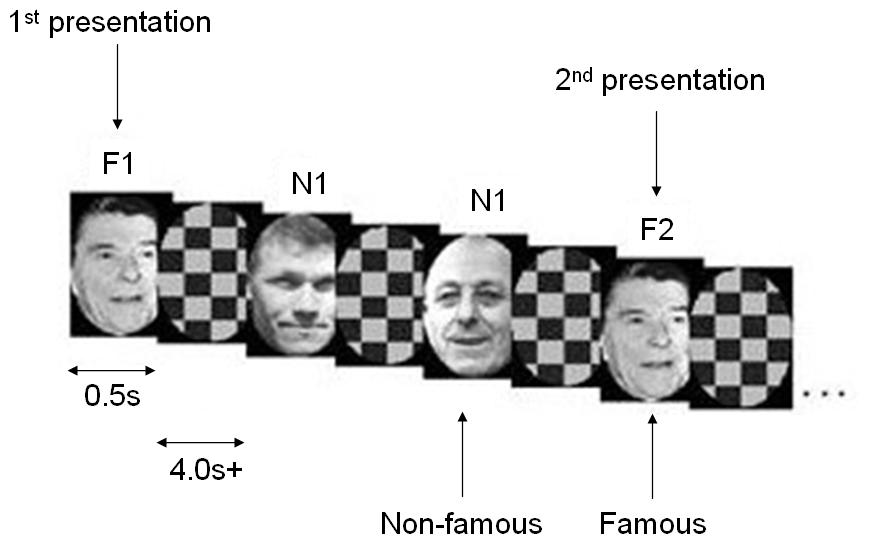
\includegraphics[width=120mm]{faces/face_stim}
\caption{\em \textbf{Face repetition paradigm}: There were 2 presentations of 26 Famous and 26 Nonfamous Greyscale photographs, for 0.5s each, randomly intermixed. The minimal Stimulus Onset Asynchrony (SOA)=4.5s, with probability 2/3 (ie 1/3 null events). The subject made one of two right finger key presses denoting whether or not the subject thought the face was famous. \label{face_stim}}
\end{center}
\end{figure}

\begin{figure}
\begin{center}
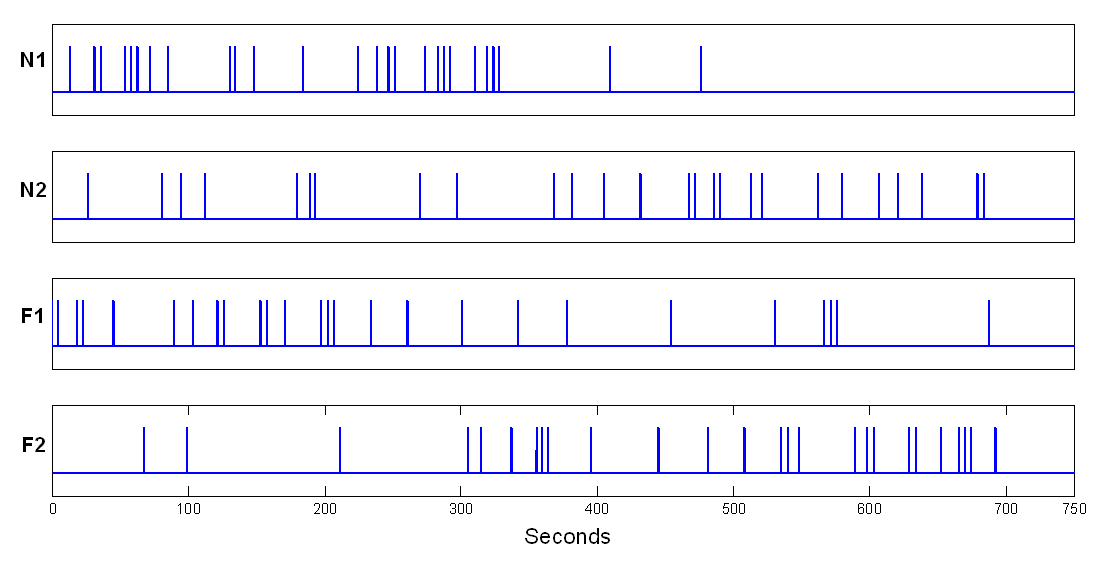
\includegraphics[width=140mm]{faces/face_timing}
\caption{\em Time series of events. \label{face_timing}}
\end{center}
\end{figure}

Images were acquired using continuous Echo-Planar Imaging (EPI) with TE=40ms, TR=2s and 24 descending slices (64$\times$64 3$\times$3 mm$^2$), 3mm thick with a 1.5mm gap.
The data archive is available from the SPM website\footnote{Face Repetition dataset: \url{http://www.fil.ion.ucl.ac.uk/spm/data/face_rep/}}.
This contains 351 Analyze format functional images \texttt{sM03953\_0005\_*.img} of dimension 64$\times$64$\times$24 with 3$\times$3$\times$4.5 mm$^3$ voxels. A structural image is also provided  in Analyze format (\texttt{sM03953\_0007.img}).

To analyse the data, first create a new directory \texttt{DIR} eg. \texttt{C:$\backslash$data$\backslash$face\_rep}, in which to place the results of your analysis. Then create 4 subdirectories (i) \texttt{jobs}, (ii) \texttt{categorical}, (iii)  \texttt{parametric} and (iv) \texttt{bayesian}. As the analysis proceeds these directories will be filled with job-specification files, design matrices and models estimated using classical or Bayesian methods. 

As well as the classical/Bayesian distinction we will show how this data can be analysed from a parametric as well as a categorical perspective. We will look at the 
main effects of fame and repetition and in the parameteric analysis we will look at responses as a function of ``lag'', that is, the number of faces intervening between repetition of a specific face.

Start up matlab, enter your jobs directory and type \texttt{spm fmri} at the \matlab\ prompt. SPM will then open in fMRI mode with three windows (1) the top-left or ``Menu'' window, (2) the bottom-left or ``Interactive'' window and (3) the right-hand or ``Graphics'' window. 
Analysis then takes place in three major stages (i) spatial pre-processing, (ii) model specification, review and estimation and (iii) inference. These stages organise the buttons in SPM's base window.
\begin{figure}
\begin{center}
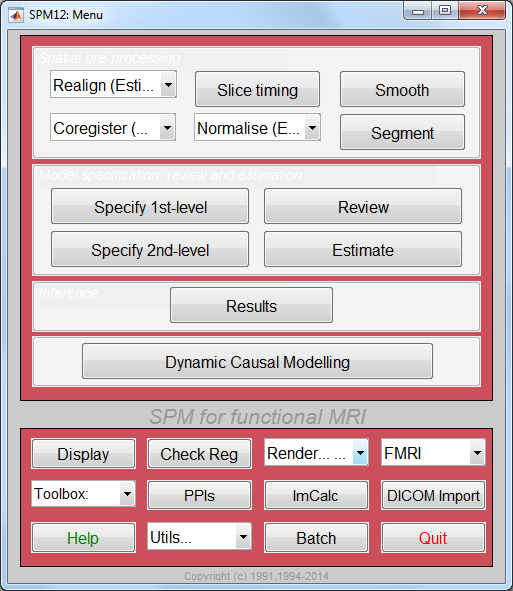
\includegraphics[width=100mm]{faces/command}
\caption{\em The SPM base window comprises three sections (i) spatial pre-processing, (ii) model specification, review and estimation and (iii) inference. \label{command}}
\end{center}
\end{figure}

\section{Spatial pre-processing}

\subsection{Display}

Display eg. the first functional image using the ``Display'' button. Note orbitofrontal and inferior temporal drop-out and ghosting. This can be seen more clearly by selecting ``brighten'' from the ``Effects'' tab in the ``Colours'' at the top of the Graphics window.

\begin{figure}
\begin{center}
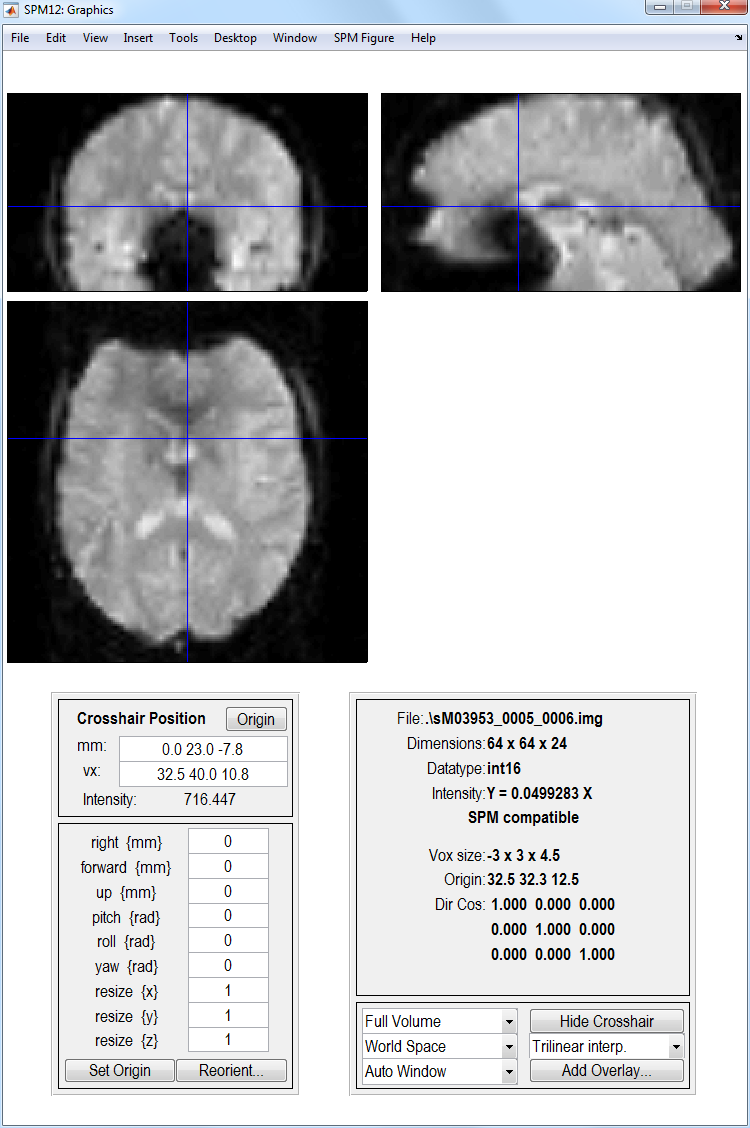
\includegraphics[width=100mm]{faces/dropout}
\caption{\em Signal dropout in EPI images. \label{dropout}}
\end{center}
\end{figure}

\subsection{Realignment}

Under the spatial pre-processing section of the SPM base window select \textsc{Realign (Est \& Res)} from the \textsc{Realign} pulldown menu. This will call up a realignment job specification in the batch editor window.
Then
\begin{itemize}
\item Highlight data, select ``New Session'', then highlight the newly created ``Session'' option.
\item Select ``Specify Files'' and use the SPM file selector to choose all of your functional images eg. \texttt{sM03953\_0005\_*.img}.
\item Save the job file as eg. \texttt{DIR/jobs/realign.mat}.
\item Press the \texttt{Rrn} button in the batch editor window (green triangle).
\end{itemize}
This will run the realign job which will write realigned images into the directory where the functional images are. These new images will be prefixed with the letter ``\texttt{r}''. SPM will then plot the estimated time series of translations and rotations shown in Figure~\ref{face_realign}. These data, the realignment parameters, are also saved to a file eg. \texttt{rp\_sM03953\_0005\_0006.txt}, so that these variables can be used as regressors when fitting GLMs. To prepare for this, copy the file into the \texttt{DIR/jobs} directory and rename it \texttt{movepars.txt}. This allows movements effects to be discounted when looking for brain activations.

SPM will also create a mean image eg. \texttt{meansM03953\_0005\_0006.img} which will be used in the next step of spatial processing - coregistration.
\begin{figure}
\begin{center}
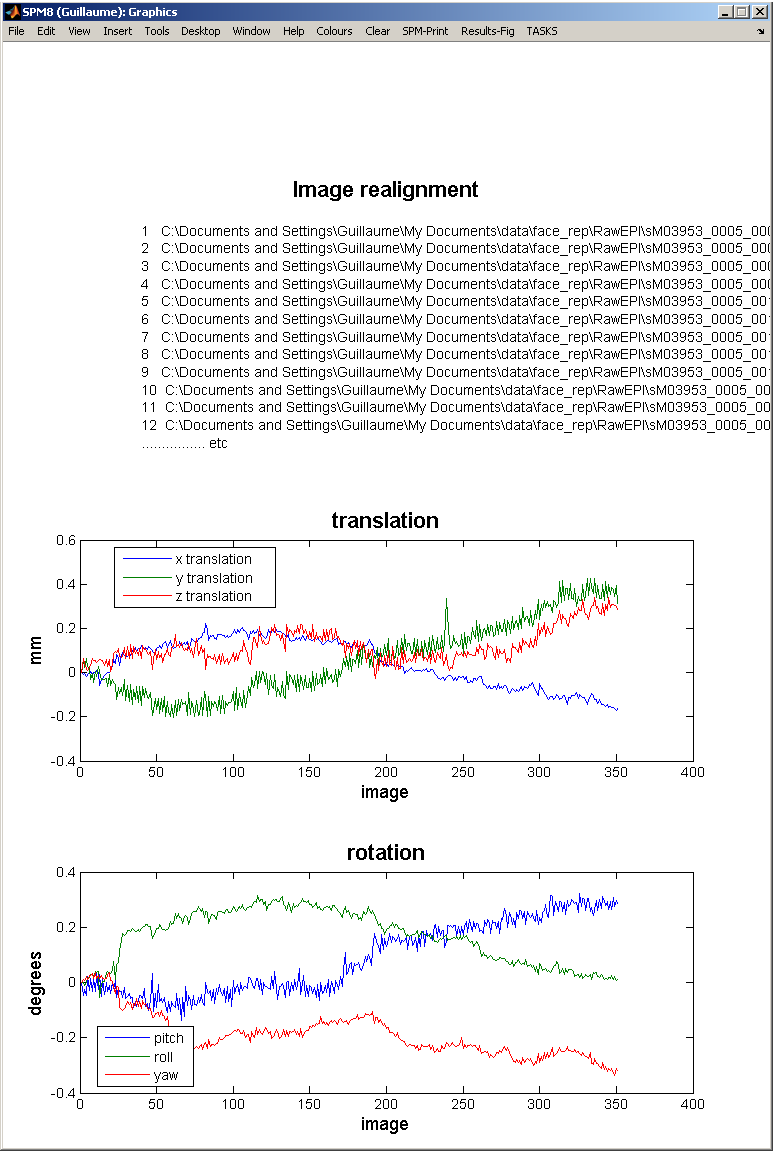
\includegraphics[width=100mm]{faces/realign}
\caption{\em \textbf{Realignment of face data}: Movement less than the size of a voxel, which for this data set is 3mm, is not considered problematic. \label{face_realign}}
\end{center}
\end{figure}

\subsection{Slice timing correction}

Press the textsc{Slice timing} button. This will call up the specification of a slice timing job in the batch editor window. Note that these data consist of N=24 axial slices acquired continuously with a TR=2s (ie TA = TR - TR/N, where TA is the time between the onset of the first and last slice of one volume, and the TR is the time between the onset of the first slice of one volume and the first slice of next volume) and in a descending order (ie, most superior slice was sampled first). The data however are ordered within the file such that the first slice (slice number 1) is the most inferior slice, making the slice acquisition order [24 23 22 ... 1].

\begin{itemize}
\item Highlight ``Data'' and select ``New Sessions''
\item Highlight the newly create ``Sessions'' option, ``Specify Files'' and select the 351 realigned functional images using the filter \texttt{\textasciicircum r.*}.
\item Select ``Number of Slices'' and enter 24.
\item Select TR and enter 2.
\item Select TA and enter 1.92 (or 2 - 2/24).
\item Select ``Slice order'' and enter 24:-1:1.
\item Select ``Reference Slice'', and enter 12.
\item Save the job as \texttt{slice\_timing.mat} and press the ``Run'' button.
\end{itemize}
SPM will write slice-time corrected files with the prefix ``\texttt{a}'' in the functional data directory.

\subsection{Coregistration}

Select \textsc{Coregister (Estimate)} from the \texttt{Coregister} pulldown menu. This will call up the specification of a coregistration job in the batch editor 
window. 

\begin{itemize}
\item Highlight ``Reference Image'' and then select the mean functional image \texttt{meansM03953\_0005\_0006.img}.
\item Highlight ``Source Image'' and then select the structural image eg. \texttt{sM03953\_0007.img}.
\item Press the ``Save'' button and save the job as \texttt{coreg.job}
\item Then press the ``Run'' button.
\end{itemize}

SPM will then implement a coregistration between the structural and functional data that maximises the mutual information. The image in figure~\ref{face_coreg} should then appear in the graphics window. SPM will have changed the header of the source file which in this case is the structural image \texttt{sM03953\_0007.img}.

\begin{figure}
\begin{center}
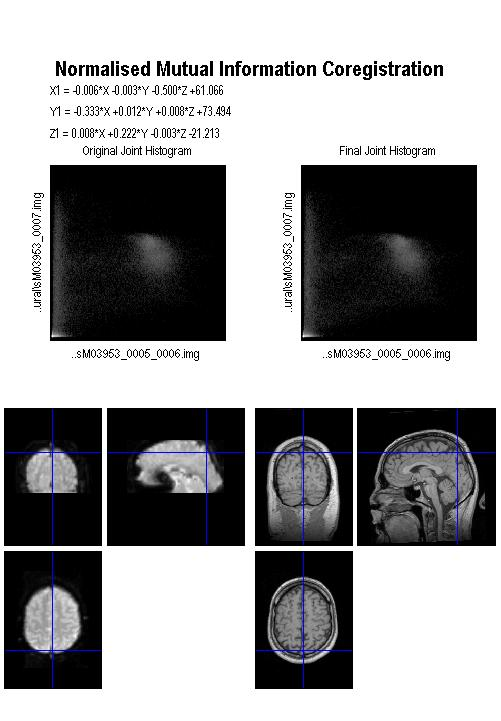
\includegraphics[width=100mm]{faces/coreg}
\caption{\em Mutual Information Coregistration of Face data.\label{face_coreg}}
\end{center}
\end{figure}

\subsection{Segmentation}

Press the \textsc{Segment} button. This will call up the specification of a segmentation job in the batch editor window. Highlight the ``Data'' field and then select the subjects coregistered anatomical image eg. \texttt{sM03953\_0007.img}. Save the job file as \texttt{segment.mat} and then press the \texttt{Run} button. SPM will segment the structural image using the default tissue probability maps as priors. 
SPM will create, by default, gray and white matter images and bias-field corrected structral image. These can be viewed using the CheckReg facility as described in the previous section. Figure~\ref{face_gray} shows the gray matter image, \texttt{c1sM03953\_0007.img}, along with the original structural\footnote{Segmentation can sometimes fail if the source (structural) image is not close in orientation to the MNI templates. It is generally advisable to manually orient the structural to match the template (ie MNI space) as close as possible by using the ``Display'' button, adjusting x/y/z/pitch/roll/yaw, and then pressing the ``Reorient'' button.}.

\begin{figure}
\begin{center}
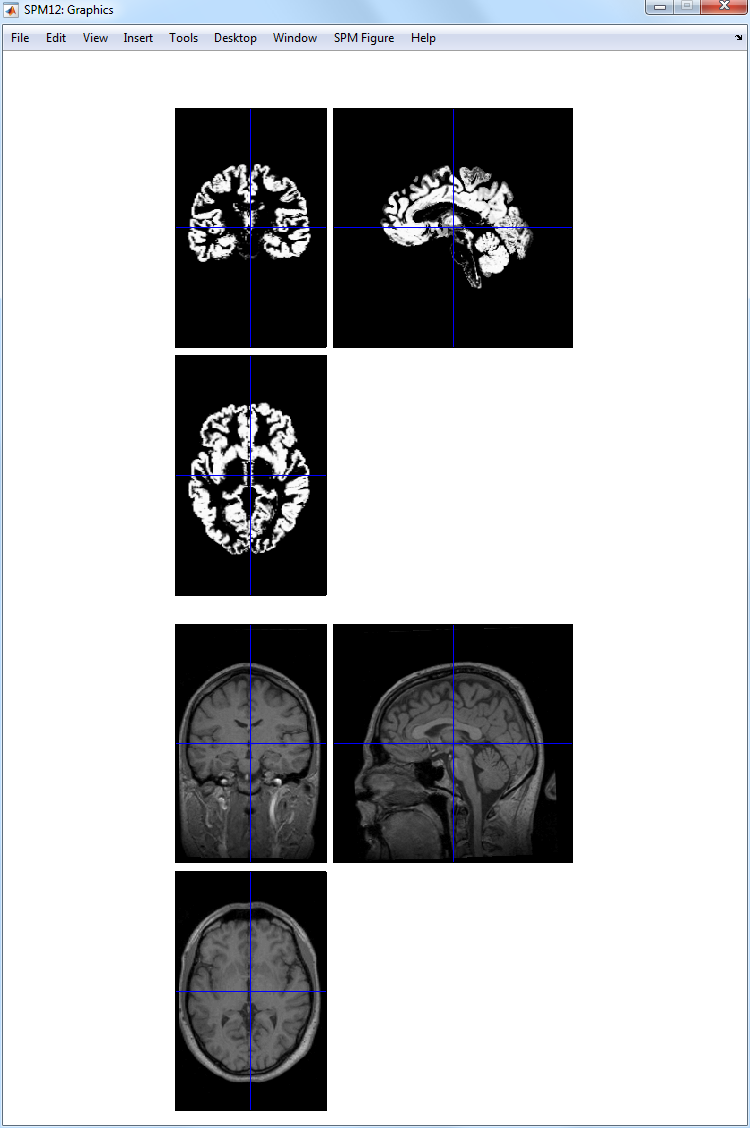
\includegraphics[width=100mm]{faces/gray}
\caption{\em Gray matter (top) produced by segmentation of structural image (below). \label{face_gray}}
\end{center}
\end{figure}

SPM will also write a spatial normalisation eg. \texttt{sM03953\_0007\_seg\_sn.mat} file in the original structural directory. This will be used in the next section to normalise the functional data. 

\subsection{Normalise}

Select \textsc{Normalise (Write)} from the \textsc{Normalise} pulldown menu. This will call up the specification of a normalise job in the batch editor window. 

\begin{itemize}
\item Highlight ``Data'', select ``New Subject''.
\item Open ``Subject'', highlight ``Parameter File'' and select the \texttt{sM03953\_0007\_seg\_sn.mat} file that you created in the previous section.
\item Highlight images to write and select all of the slice-time corrected, realigned functional images \texttt{arsM*.img}. Note: This can be done efficiently by changing the filter in the SPM file selector to \texttt{\textasciicircum ar.*}. You can then right click over the listed files, choose ``Select all''. You might also want to select the mean functional image created during realignment (which would not be affected by slice-time correction), i.e, the \texttt{meansM03953\_0005\_006.img}. Then press ``Done''.
\item Open ``Writing Options'', and change ``Voxel sizes'' from [2 2 2] to [3 3 3]\footnote{This step is not strictly necessary. It will write images out at a resolution closer to that at which they were acquired. This will speed up subsequent analysis and is necessary, for example, to make Bayesian fMRI analysis computationally efficient.}.
\item Press ``Save'', save the job as normalise.mat and then press the \texttt{Run} button.
\end{itemize}
SPM will then write spatially normalised files to the functional data directory. These files have the prefix ``\texttt{w}''.

If you wish to superimpose a subject's functional activations on their own anatomy\footnote{Beginners may wish to skip this step, and instead just superimpose functional activations on an ``canonical structural image''.} you will also need to apply the spatial normalisation parameters to their (bias-corrected) anatomical image. To do this
\begin{itemize}
\item Select \textsc{Normalise (Write)}, highlight `Data', select ``New Subject''.
\item Highlight ``Parameter File'', select the \texttt{sM03953\_0007\_seg\_sn.mat} file that you created in the previous section, press ``Done''.
\item Highlight ``Images to Write'', select the bias-corrected structural eg. \texttt{msM03953\_0007.img}, press ``Done''.
\item Open ``Writing Options'', select voxel sizes and change the default [2 2 2] to [1 1 1] which better matches the original resolution of the images [1 1 1.5].
\item Save the job as \texttt{norm\_struct.mat} and press \texttt{Run} button.
\end{itemize}

\subsection{Smoothing}

Press the \textsc{Smooth} button\footnote{The smoothing step is unnecessary if you are only interested in Bayesian analysis of your functional data.}. This will call up the specification of a smooth job in the batch editor window.

\begin{itemize}
\item Select ``Images to Smooth'' and then select the spatially normalised files created in the last section eg. \texttt{war*.img}.
\item Save the job as {\sf smooth.mat} and press \texttt{Run} button.
\end{itemize}

This will smooth the data by (the default) 8mm in each direction, the default smoothing kernel width.

\begin{figure}
\begin{center}
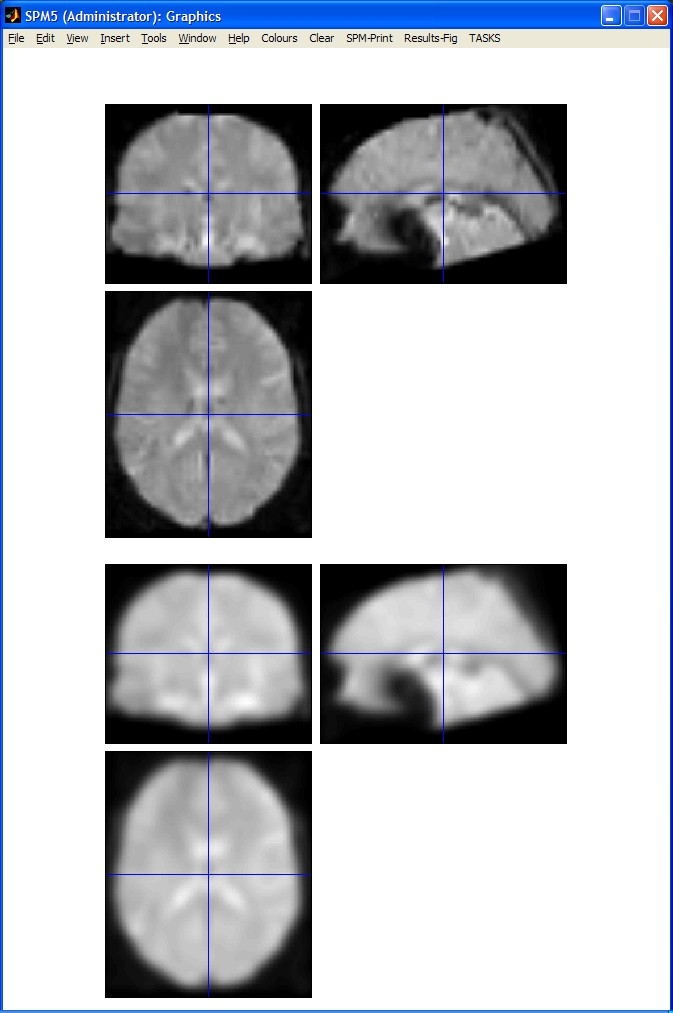
\includegraphics[width=100mm]{faces/smooth}
\caption{\em Functional image (top) and 8mm-smoothed functional image (bottom). These images were plotted using SPM's ``CheckReg'' facility. \label{face_smooth}}
\end{center}
\end{figure}

\section{Modelling categorical responses}

Before setting up the design matrix we must first load the Stimulus Onsets Times (SOTs) and movement parameters into matlab. SOTs are stored in the \texttt{sots.mat} file in a cell array such that eg. \texttt{sot\{1\}} contains stimulus onset times in TRs for event type 1, which is N1. Event-types 2, 3 and 4 are N2, F1 and F2.\footnote{Unlike previous analyses of these data in SPM99 and SPM2, we will not bother with extra event-types for the (rare) error trials.}
\begin{itemize}
\item At the \matlab\ command prompt type \texttt{load sots}
\item Then type \texttt{load movepars.txt}
\end{itemize}

Now press the \textsc{Specify 1st-level} button. This will call up the specification of a fMRI specification job in the batch editor window. Then

\begin{itemize}
\item In the ``Timing paramaters'' option,
\item Highlight ``Units for design'' and select ``Scans'',
\item Highlight ``Interscan interval'' and enter 2,
\item Highlight ``Microtime resolution'' and enter 24,
\item Highlight ``Microtime onset'' and enter 12. These last two options make the creating of regressors commensurate with the slice-time correction we have applied to the data, given that there are 24 slices and that the reference slice to which the data were slice-time corrected was the 12th (middle slice in time).
\item Highlight ``Data and Design'' and select ``New Subject/Session''.
\item Highlight ``Scans'' and use SPM's file selector to choose the 351 smoothed, normalised, slice-time corrected, realigned functional images ie \texttt{swarsM.img}. These can be selected easily using the \texttt{\textasciicircum swar.*} filter, and select all. Then press ``Done''.
\item Highlight ``Conditions'' and select ``New condition''\footnote{It is also possible to enter information about all of the conditions in one go. This requires much less button pressing and can be implemented by highlighting the ``Multiple conditions'' option and then selecting the \texttt{all-conditions.mat} file, which is also provided on the webpage.}.
\item Open the newly created ``Condition'' option. Highlight ``Name'' and enter ``N1''. Highlight ``Onsets'' and enter \texttt{sot\{1\}}. Highlight ``Durations'' and enter 0.
\item Highlight ``Conditions'' and select ``Replicate condition''.
\item Open the newly created ``Condition'' option (the lowest one). Highlight ``Name'' and change to ``N2''. Highlight ``Onsets'' and enter \texttt{sot\{2\}}.
\item Highlight ``Conditions'' and select ``Replicate condition''.
\item Open the newly created ``Condition'' option (the lowest one). Highlight ``Name'' and change to ``F1''. Highlight ``Onsets'' and enter \texttt{sot\{3\}}.
\item Highlight ``Conditions'' and select ``Replicate condition''.
\item Open the newly created ``Condition'' option (the lowest one). Highlight ``Name'' and change to ``F2''. Highlight ``Onsets'' and enter \texttt{sot\{4\}}.
\item Highlight ``Multiple Regressors'' and select the \texttt{movepars.txt} file\footnote{It is also possible to enter regressors one by one by highlighting ``Regressors'' and selecting ``New Regressor'' for each one. Here, we benefit from the fact that the realignment stage produced a text file with the correct number of rows (351) and columns (6) for SPM to add 6 regressors to model (linear) rigid-body movement effects.}.
\item Highlight ``Factorial Design'', select ``New Factor'', open the newly created ``Factor'' option, highlight ``Name'' and enter ``Fam'', highlight ``Levels'' and enter 2.
\item Highlight ``Factorial Design'', select ``New Factor'', open the newly created ``Factor'' option, highlight ``Name'' and enter ``Rep'', highlight ``Levels'' and enter 2\footnote{The order of naming these factors is important - the factor to be specified first is the one that ``changes slowest'' ie. as we go through the list of conditions N1, N2, F1, F2 the factor ``repetition'' changes every condition and the factor ``fame'' changes every other condition. So ``Fam'' changes slowest and is entered first.}.
\item Open ``Canonical HRF'' under ``Basis Functions''. Select ``Model derivatives'' and select ``Time and Dispersion derivatives''.
\item Highlight ``Directory'' and select the \texttt{DIR/categorical} directory you created earlier.
\item Save the job as \texttt{categorical\_spec.mat} and press the \texttt{Run} button.
\end{itemize}

SPM will then write an \texttt{SPM.mat} file to the \texttt{DIR/categorical} directory. It will also plot the design matrix, as shown in Figure~\ref{cat_design}. 
\begin{figure}
\begin{center}
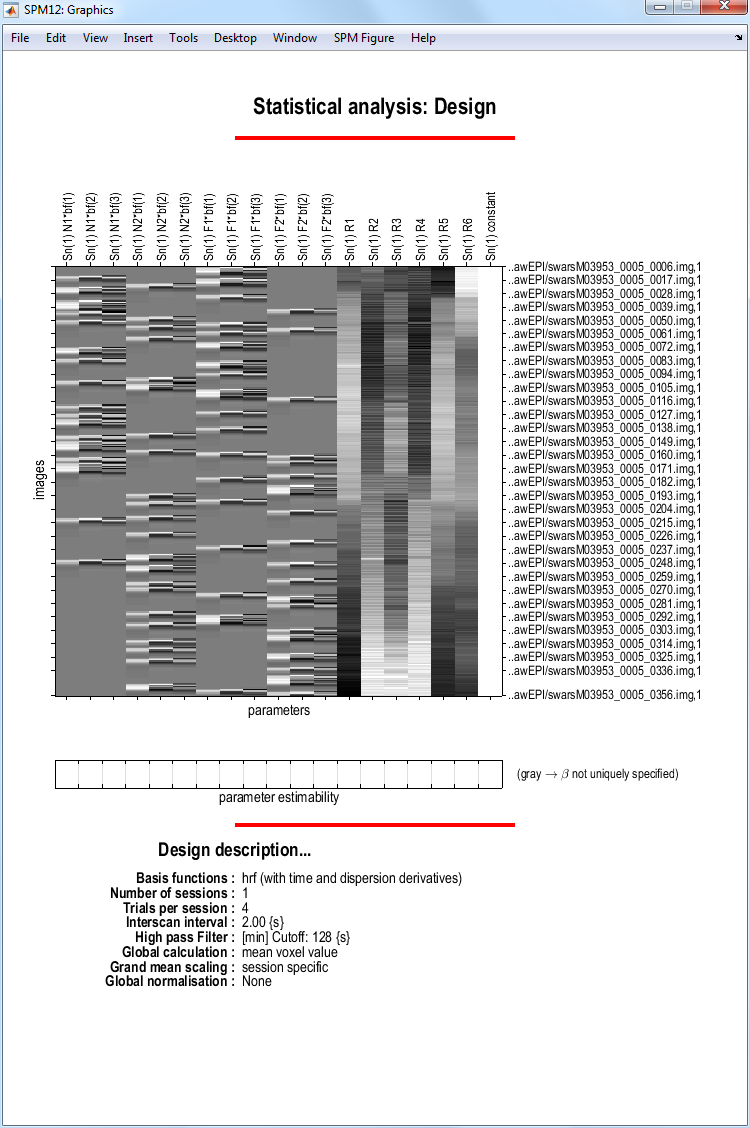
\includegraphics[width=100mm]{faces/cat_design}
\caption{\em \textbf{Design matrix}. \label{cat_design}}
\end{center}
\end{figure}

At this stage it is advisable to check your model specification using SPM's review facility which is accessed via the ``Review'' button. This brings up a ``design'' tab on the interactive window clicking on which produces a pulldown menu. If you select the first item ``Design Matrix'' SPM will produce the image shown in Figure~\ref{cat_design}. If you select ``Explore'' then ``Session 1'' then ``N1'', SPM will produce the plots shown in Figure~\ref{cat_explore}.
\begin{figure}
\begin{center}
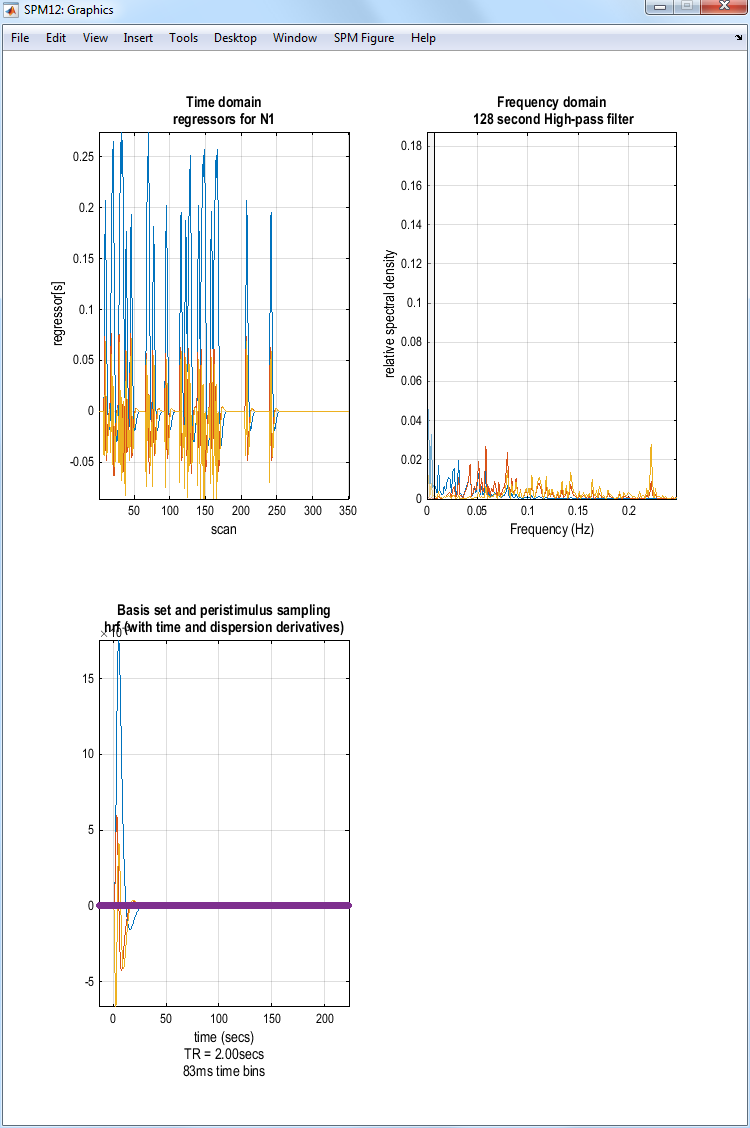
\includegraphics[width=100mm]{faces/cat_explore}
\caption{\em \textbf{Exploring the design matrix in Figure~\ref{cat_design}}. This shows the time series of the ``N1'' regressor (top left), the three basis functions used to convert assumed neuronal activity into hemodynamic activity (bottom left), and a frequency domain plot of the three regressors for the basis functions in this condition (top right). The frequency domain plot shows that the frequency content of the ``N1'' condition is generally above the set frequencies that are removed by the High Pass Filter (HPF) (these are shown in gray - in this model we accepted the default HPF cut-off of 128s or 0.008Hz). \label{cat_explore}}
\end{center}
\end{figure}

\subsection{Estimate}

Press the \textsc{Estimate} button. This will call up the specification of an fMRI estimation job in the batch editor window. Then
\begin{itemize}
\item Highlight the ``Select SPM.mat'' option and then choose the \texttt{SPM.mat} file saved in the \texttt{DIR/categorical} directory.
\item Save the job as \texttt{categorical\_est.job} and press \texttt{Run} button.
\end{itemize}
SPM will write a number of files into the selected directory including an \texttt{SPM.mat} file.

\subsection{Inference for categorical design}

Press ``Results'' and select the SPM.mat file from \texttt{DIR/categorical}. This will again invoke the contrast manager. Because we specified that our model was using a ``Factorial design'' a number of contrasts have been specified automatically, as shown in Figure~\ref{cat_contrasts}.
\begin{figure}
\begin{center}
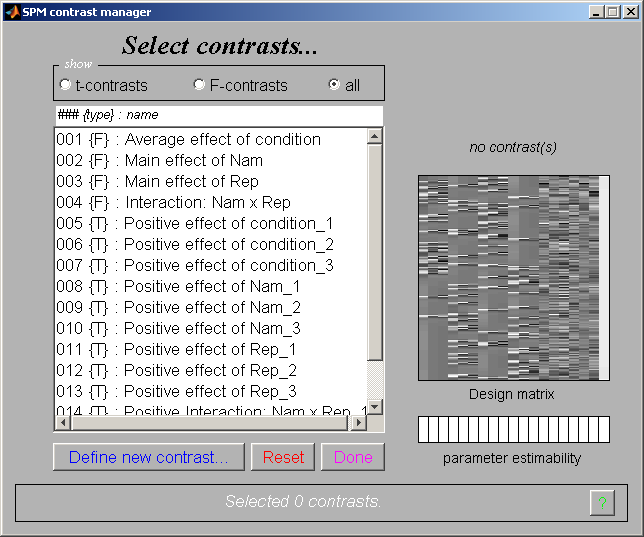
\includegraphics[width=100mm]{faces/cat_contrasts}
\caption{\em Contrast Manager containing default contrasts for categorical design. \label{cat_contrasts}}
\end{center}
\end{figure}

\begin{itemize}
\item Select contrast number 5. This is a t-contrast \texttt{Positive effect of condition\_1} This will show regions where the average effect of presenting faces is significantly positive, as modelled by the first regressor (hence the \texttt{\_1}), the canonical HRF. Press `Done''.
\item \emph{Mask with other contrast ? [Yes/No]}
\item Specify No.
\item \emph{Title for comparison ?}
\item Enter ``Canonical HRF: Faces $>$ Baseline''
\item \emph{p value adjustment to control: [FWE/FDR/none]}
\item Select FWE
\item \emph{Corrected p value(family-wise error)}
\item Accept the default value, 0.05
\item \emph{Extent threshold \{voxels\} [0]}
\item Accept the default value, 0.
\end{itemize}
SPM will then produce the MIP shown in Figure~\ref{cat5_volume}.

\subsection{Statistical tables}

To get a summary of local maxima, press the ``whole brain'' button in the p-values section of the interactive window. This will list all clusters above the chosen level of significance as well as separate ($>$8mm apart) maxima within a cluster, with details of significance thresholds and search volume underneath, as shown in Figure~\ref{cat5_volume}
\begin{figure}
\begin{center}
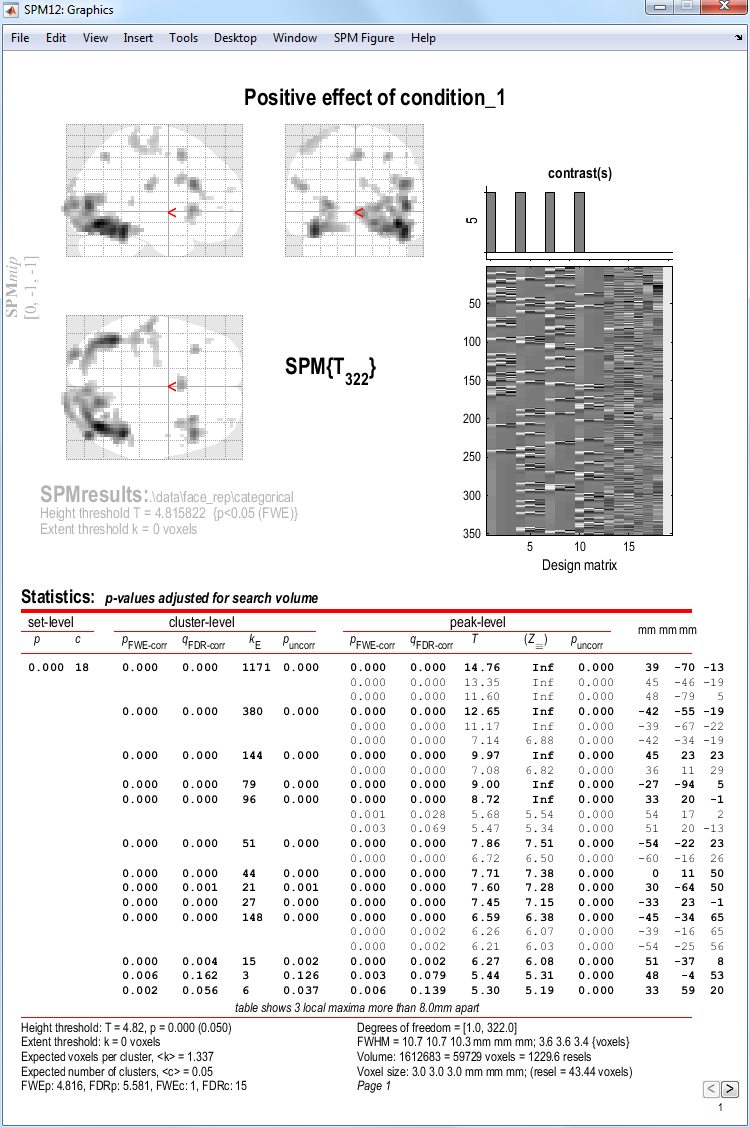
\includegraphics[width=100mm]{faces/cat5_volume}
\caption{\em \textbf{MIP and Volume table for Canonical HRF}: Faces  $>$ Baseline. \label{cat5_volume} }
\end{center}
\end{figure}

The columns in volume table show, from right to left:
\begin{itemize}
\item \textbf{x, y, z (mm)}: coordinates in MNI space for each maximum.
\item \textbf{peak-level}: the chance (p) of finding (under the null hypothesis) a peak with this or a greater height (T- or Z-statistic), corrected (FWE or FDR)/ uncorrected for search volume.
\item \textbf{cluster-level}: the chance (p) of finding a cluster with this many(ke) or a greater number of voxels, corrected (FWE or FDR)/ uncorrected for search volume.
\item \textbf{set-level}: the chance (p) of finding this (c) or a greater number of clusters in the search volume.
\end{itemize}

Right-click on the MIP and select ``goto global maximum''. The cursor will move to [39 -70 -14]. You can view this activation on the subject's normalised, attenuation-corrected structural (\texttt{wmsM03953\_0007\.img}), which gives best anatomical precision, or on the normalised mean functional (\texttt{wmeansM03953\_0005\_0006.img}), which is closer to the true data and spatial resolution (including distortions in the functional EPI data). 

If you select ``plot'' and choose ``Contrast of estimates and 90\% C.I'' (confidence interval), and select the ``Average effect of condition'' contrast, you will see three bars corresponding to the parameter estimates for each basis function (summed across the 4 conditions). The BOLD impulse response in this voxel loads mainly on the canonical HRF, but also significantly (given that the error bars do not overlap zero) on the temporal and dispersion derivatives (see next Chapter).

\subsection{F-contrasts}

To assess the main effect of repeating faces, as characterised by both the hrf \emph{and} its derivatives, an F-contrats is required. This is really asking whether repetition changes the \emph{shape} of the impulse response (e.g, it might affect its latency but not peak amplitude), at least the range of shapes defined by the three basis functions. Because we have told SPM that we have a factorial design, this required contrast will have been created automatically - it is number 3. 

\begin{itemize}
\item Press ``Results'' and select the \texttt{SPM.mat} file in the \texttt{DIR/categorical} directory.
\item Select the ``F-contrast'' toggle and the contrast number 3, as shown in Figure~\ref{cat3_contrast}. Press ``Done''.
\item \emph{Mask with other contrast ? [Yes/No]}.
\item Specify ``Yes''.
\item Select contrast 5 - \texttt{Positive effect of condition\_1} (the T-contrast of activation versus baseline, collapsed across conditions, that we evaluated above)
\item \emph{uncorrected mask p-value ?}
\item Change to 0.001
\item \emph{nature of mask?}
\item Select 'inclusive'
\item \emph{Title for comparison ?}
\item Keep ``Main effect of Rep (masked with ...)''
\item \emph{p value adjustment to control: [FWE/none]}
\item Select none
\item \emph{threshold (F or p value)}
\item Accept the default value, 0.001
\item \emph{Extent threshold \{voxels\} [0]}
\item Accept the default value, 0
\end{itemize}

A MIP should then appear, the top half of which should look like Figure~\ref{cat3_psth}.

\begin{figure}
\begin{center}
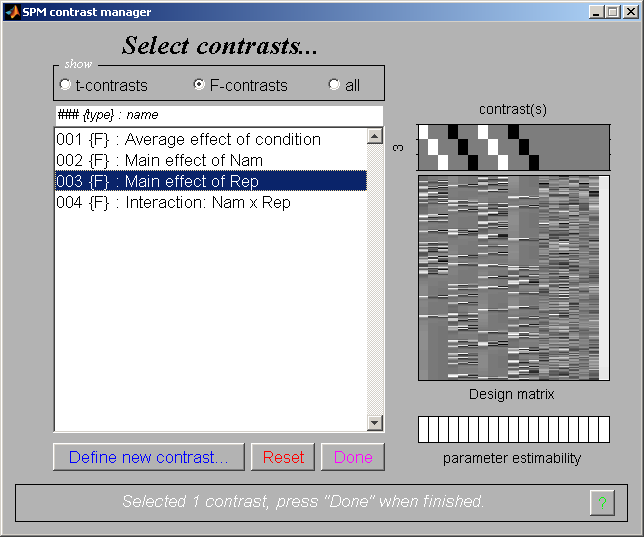
\includegraphics[width=100mm]{faces/cat3_contrast}
\caption{\em Contrast manager showing selection of the first contrast ``Main effect of Rep'' (repetition: F1 and N1 vs F2 and N2)\label{cat3_contrast} }
\end{center}
\end{figure}

\begin{figure}
\begin{center}
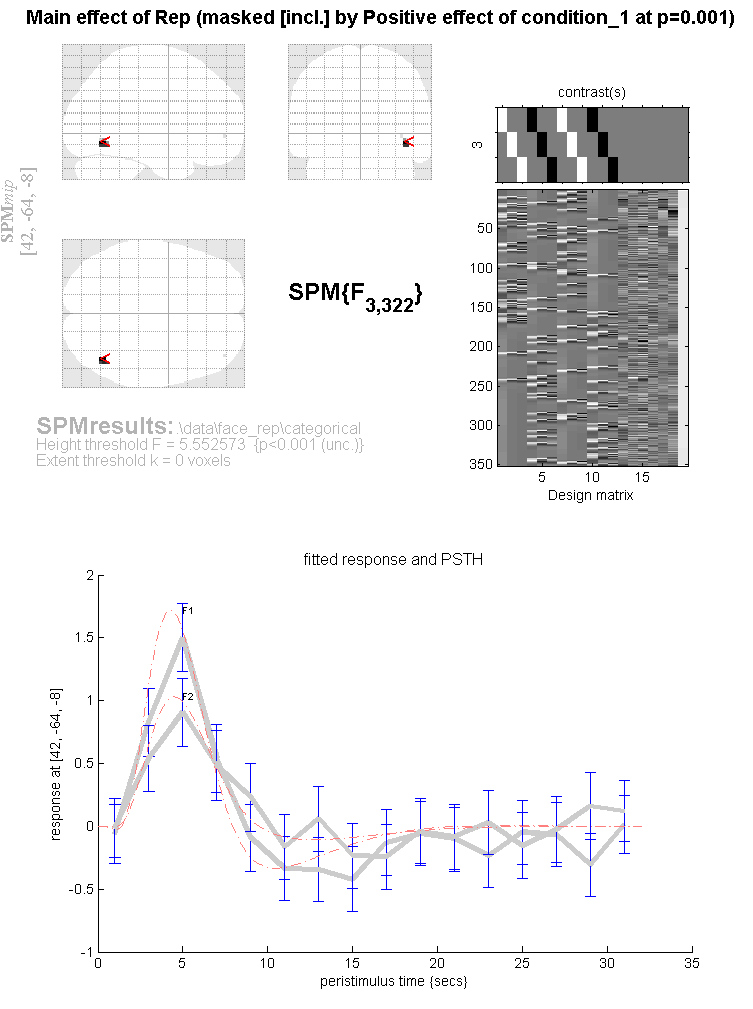
\includegraphics[width=100mm]{faces/cat3_psth}
\caption{\em MIP for Main effect of Rep, masked inclusively with Canonical HRF: Faces  $>$ Baseline at p$<$.001 uncorrected. Shown below are the best-fitting responses and peri-stimulus histograms (PSTH) for F1 and F2. \label{cat3_psth} } 
\end{center}
\end{figure}

Note that this contrast will identify regions showing any effect of repetition (e.g, decreased or increased amplitudes) \emph{within} those regions showing activations (on the canonical HRF) to faces versus baseline (at p$<$.05 uncorrected). Select ``goto global max'', which is in right ventral temporal cortex [42 -64 -8].

If you press plot and select ``Event-related responses'', then ``F1'', then ``fitted response and PSTH'', you will see the best fitting linear combination of the canonical HRF and its two derivatives (thin red line), plus the ``selectively-averaged'' data (peri-stimulus histogram, PSTH), based on an FIR refit (see next Chapter). 
If you then select the ``hold'' button on the Interactive window, and then ``plot'' and repeat the above process for the ``F2'' rather than ``F1'' condition, you will see two estimated event-related responses, in which repetition decreases the peak response (ie F2$<$F1), as shown in Figure~\ref{cat3_psth}.

You can explore further F-contrasts, which are a powerful tool once you understand them. For example, the MIP produced by the ``Average effect of condition'' F-contrast looks similar to the earlier T-contrast, but importantly shows the areas for which the sums across conditions of the parameter estimates for the canonical hrf \emph{and/or} its temporal derivative \emph{and/or} its dispersion derivative are different from zero (baseline). The first row of this F-contrast ([1 0 0 1 0 0 1 0 0 1 0 0]) is also a two-tailed version of the above T-contrast, ie testing for both activations and deactivations versus baseline. This also means that the F-contrasts [1 0 0 1 0 0 1 0 0 1 0 0] and [-1 0 0 -1 0 0 -1 0 0 -1 0 0] are equivalent. Finally, note that an F- (or t-) contrast such as [1 1 1 1 1 1 1 1 1 1 1], which tests whether the mean of the canonical hrf AND its derivatives for all conditions are different from (larger than) zero is not sensible. This is because the canonical hrf and its temporal derivative may cancel each other out while being significant in their own right. The basis functions are really quite different things, and need to represent separate rows in an F-contrast. 

\subsection{F-contrasts for testing effects of movement}

To assess movement-related activation
\begin{itemize}
\item Press ``Results'', select the \texttt{SPM.mat} file, select ``F-contrast'' in the Contrast Manager. Specify e.g. ``Movement-related effects'' (name) and 
in the ``contrasts weights matrix'' window, or ``1:12 19'' in the ``columns for reduced design'' window.
\item Submit and select the contrast, specify ``mask with other contrasts?'' (no), ``title for comparison'' (accept default), ``corrected height threshold'' (FWE), and ``corrected p-value'' (accept default). 
\item When the MIP appears, select ``sections'' from the ``overlays'' pulldown menu, and select the normalised structural image (\texttt{wmsM03953\_0007.img}).
\end{itemize}

You will see there is a lot of residual movement-related artifact in the data (despite spatial realignment), which tends to be concentrated near the boundaries of tissue types (eg the edge of the brain; see Figure~\ref{movements}). (Note how the MIP can be misleading in this respect, since though it appears that the whole brain is affected, this reflects the nature of the (X-ray like) projections onto each orthogonal view; displaying the same datae as sections in 3D shows that not every voxel is suprathreshold.)  Even though we are not interested in such artifact, by including the realignment parameters in our design matrix, we ``covary out'' (linear components) of subject movement, reducing the residual error, and hence improve our statistics for the effects of interest.

\begin{figure}
\begin{center}
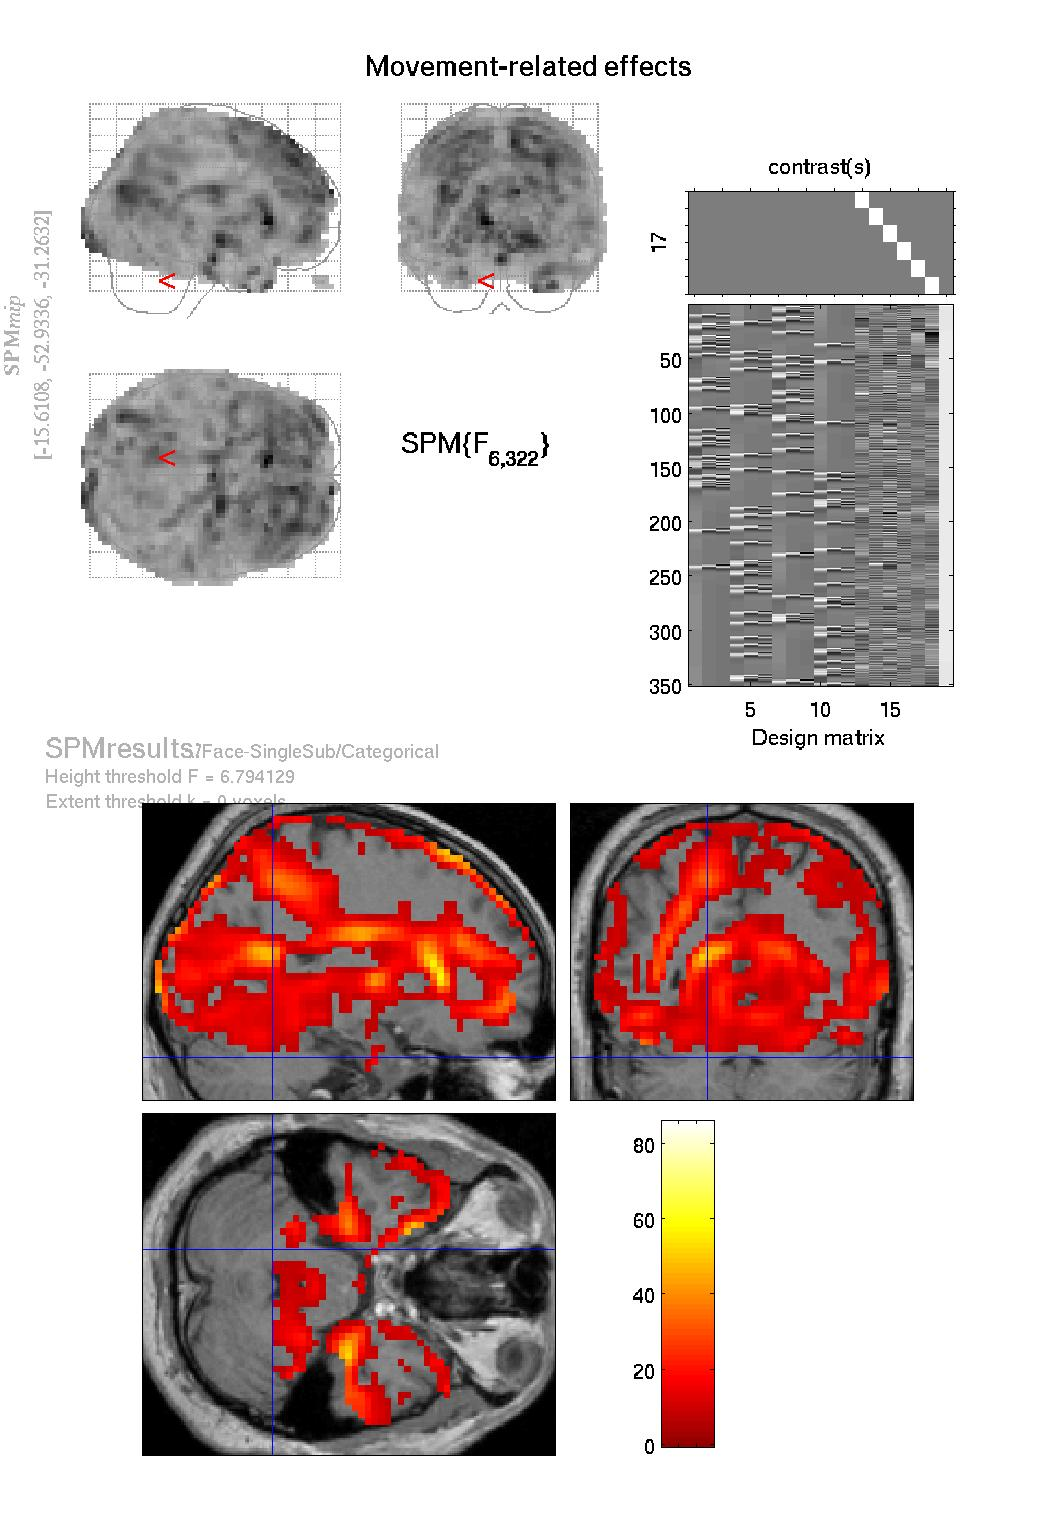
\includegraphics[width=100mm]{faces/movements}
\caption{\em Movement-related activations. These spurious `activations' are due to residual movement of the head during scanning. These effects occur at tissue boundaries and boundaries between brain and non-brain, as this is where contrast differences are greatest. Including these regressors in the design matrix means these effects cannot be falsely attributed 
to neuronal activity. \label{movements} }
\end{center}
\end{figure}

\section{Modelling parametric responses}

Before setting up the design matrix, we must first load into \matlab\ the Stimulus Onsets Times (SOTs), as before, and also the ``Lags'', which are specific to this experiment, and which will be used as parametric modulators. The Lags code, for each second presentation of a face (N2 and F2), the number of other faces intervening between this (repeated) presentation and its previous (first) presentation. Both SOTs and Lags are represented by Matlab cell arrays, stored in the \texttt{sots.mat} file.

\begin{itemize}
\item At the \matlab\ command prompt type \texttt{load sot}. This loads the stimulus onset times and the lags (the latter in a cell array called \texttt{itemlag}.
\end{itemize}

Now press the \textsc{Specify 1st-level} button. This will call up the specification of a fMRI specification job in the batch editor window. Then
\begin{itemize}
\item Press ``Load'' and select the \texttt{categorical\_spec.mat} job file you created earlier.
\item Open ``Conditions'' and then open the second ``Condition''.
\item Highlight ``Parametric Modulations'', select ``New Parameter''.
\item Highlight ``Name'' and enter ``Lag'', highlight values and enter \texttt{itemlag\{2\}}, highlight polynomial expansion and ``2nd order''.
\item Now open the fourth ``Condition'' under ``Conditions''.
\item Highlight ``Parametric Modulations'', select ``New Parameter''.
\item Highlight ``Name'' and enter ``Lag'', highlight values and enter \texttt{itemlag\{4\}}, highlight polynomial expansion and ``2nd order''.
\item Open ``Canonical HRF'' under ``Basis Functions'', highlight ``Model derivatives'' and select ``No derivatives'' (to make the design matrix a bit simpler for present purposes!).
\item Highlight ``Directory'' and select \texttt{DIR/parametric} (having ``unselected'' the current definition of directory from the Categorical analysis).
\item Save the job as \texttt{parametric\_spec} and press the \texttt{Run} button.
\end{itemize}

This should produce the design matrix shown in Figure~\ref{par_design}.

\begin{figure}
\begin{center}
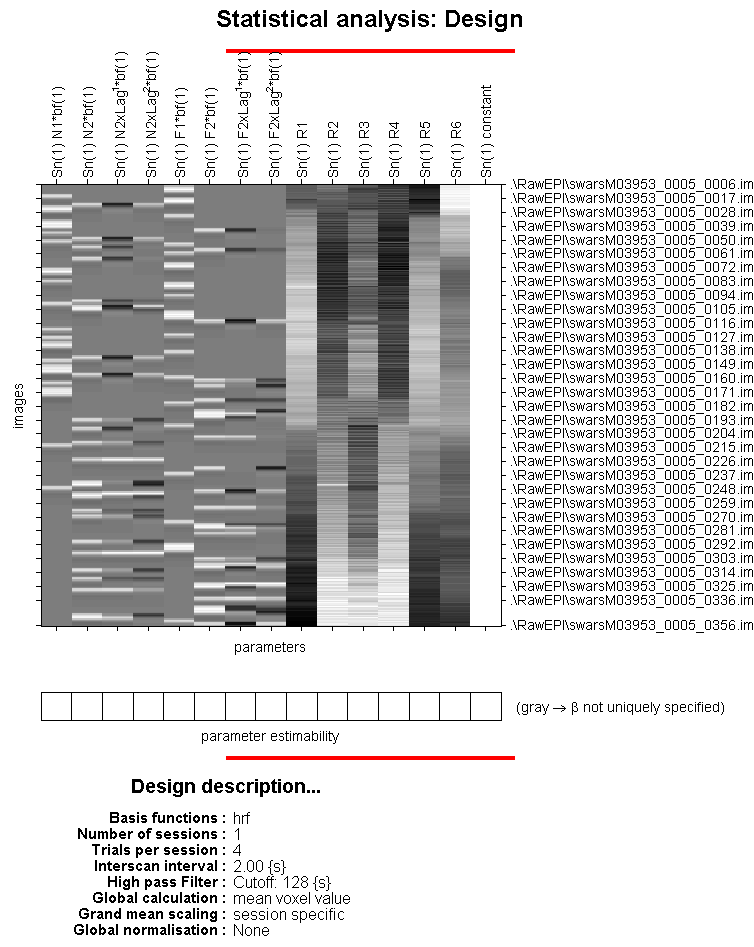
\includegraphics[width=100mm]{faces/par_design}
\caption{\em \textbf{Design matrix for testing repetition effects parametrically.} Regressor 2 indicates the second occurence of a nonfamous face. Regressor 3 modulates this linearly as a function of lag (ie. how many faces have been shown since that face was first presented), and regressor 4 modulates this quadratically as a function of lag. Regressors 6,7 and 8 play the same roles, but for famous faces. \label{par_design} }
\end{center}
\end{figure}

\subsection{Estimate}

Press the \textsc{Estimate} button. This will call up the specification of an fMRI estimation job in the batch editor window. Then
\begin{itemize}
\item Highlight the ``Select SPM.mat'' option and then choose the \texttt{SPM.mat} file saved in the \texttt{DIR/parametric} directory.
\item Save the job as \texttt{parametric\_est.job} and press the \texttt{Run} button.
\end{itemize}
SPM will write a number of files into the selected directory including an \texttt{SPM.mat} file.

\subsection{Plotting parametric responses}

We will look at the effect of lag (up to second order, ie using linear and quadratic terms) on the response to repeated Famous faces, within those regions generally activated by faces versus baseline. To do this
\begin{itemize}
\item Press ``Results'' and select the \texttt{SPM.mat} file in the \texttt{DIR/parametric} directory.
\item Press ``Define new contrast'', enter the name ``Famous Lag'', press the ``F-contrast'' radio button, enter ``1:6 9:15'' in the ``columns in reduced design'' window, press ``submit'', ``OK'' and ``Done''.
\item Select the ``Famous Lag'' contrast.
\item \emph{Mask with other contrast ? [Yes/No]}
\item Specify ``Yes''.
\item Select the ``Positive Effect of Condition 1'' T contrast.
\item Change to an 0.05 uncorrected mask p-value.
\item Nature of Mask ? inclusive.
\item \emph{ Title for comparison ?}
\item Accept what is offered
\item \emph{p value adjustment to control: [FWE/none]}
\item Select None
\item \emph{Threshold \{F or p value\}}
\item Accept the default value, 0.001
\item \emph{Extent threshold \{voxels\} [0]}
\item Accept the default value, 0.
\end{itemize}

Figure~\ref{famous_lag_mip} shows the MIP and an overlay of this parametric effect using overlays, sections and selecting the \texttt{wmsM03953\_0007.img} image. 
\begin{figure}
\begin{center}
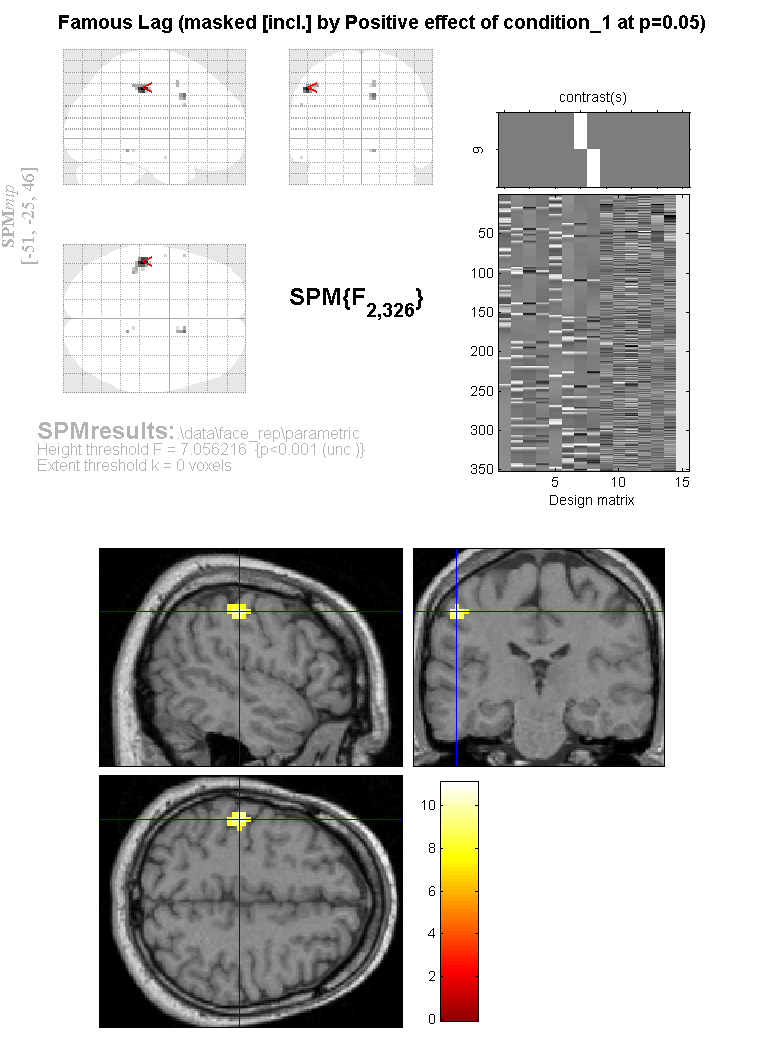
\includegraphics[width=100mm]{faces/famous_lag_mip}
\caption{\em MIP and overlay of parametric lag effect in parietal cortex. \label{famous_lag_mip} }
\end{center}
\end{figure}
The effect is plotted in the time domain in figure~\ref{famous_lag}. This was obtained by
\begin{itemize}
\item Right clicking on the MIP and selecting ``global maxima''.
\item Pressing Plot, and selecting ``parametric responses'' from the pull-down menu.
\item Which effect ? select ``F2''.
\end{itemize}

This shows a quadratic effect of lag, in which the response appears negative for short-lags, but positive and maximal for lags of about 40 intervening faces (note that this is a very approximate fit, since there are not many trials, and is also confounded by time during the session, since longer lags necessarily occur later (for further discussion of this issue, see the SPM2 example analysis of these data on the webpage).

\begin{figure}
\begin{center}
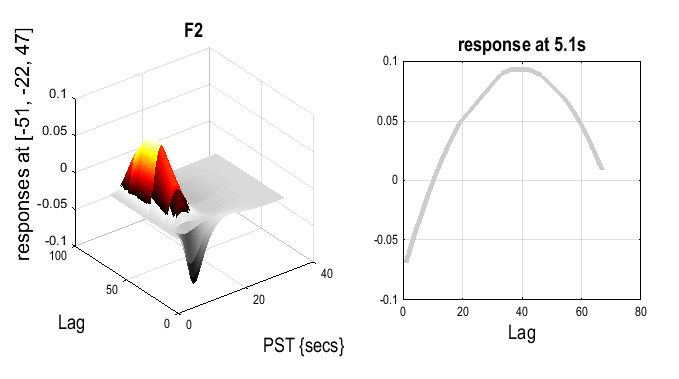
\includegraphics[width=150mm]{faces/famous_lag}
\caption{\em Response as a function of lag. \label{famous_lag} }
\end{center}
\end{figure}


\section{Bayesian analysis}

\subsection{Specification}

Press the \textsc{Specify 1st-level} button. This will call up an fMRI specification job in the batch editor window. Then

\begin{itemize}
\item Load the \texttt{categorical\_spec.mat} job file created for the classical analysis.
\item Open ``Subject/Session'', highlight ``Scans''.
\item Deselect the smoothed functional images using the `unselect all' option available from a right mouse click in the SPM file selector (bottom window).
\item Select the unsmoothed functional images using the \texttt{\textasciicircum wa.*} filter and ``select all'' option available from a right mouse click in the SPM file selector (top right window). The Bayesian analysis uses a spatial prior where the spatial regularity in the signal is estimated from the data. It is therefore not necessary to create smoothed images if you are only going to do a Bayesian analysis.
\item Press ``Done''.
\item Highlight ``Directory'' and select the \texttt{DIR/bayesian} directory you created earlier (you will first need to deselect the \texttt{DIR/categorical} directory).
\item Save the job as \texttt{specify\_bayesian.mat} and press the \texttt{Run} button.
\end{itemize}

\subsection{Estimation}

Press the \textsc{Estimate} button. This will call up the specification of an fMRI estimation job in the batch editor window. Then
\begin{itemize}
\item Highlight the ``Select SPM.mat'' option and then choose the \texttt{SPM.mat} file saved in the \texttt{DIR/bayesian} subdirectory
\item Highlight ``Method'' and select the ``Choose Bayesian 1st-level'' option.
\item Save the job as \texttt{estimate\_bayesian.job} and press the \texttt{Run} button.
\end{itemize}

\begin{figure}
\begin{center}
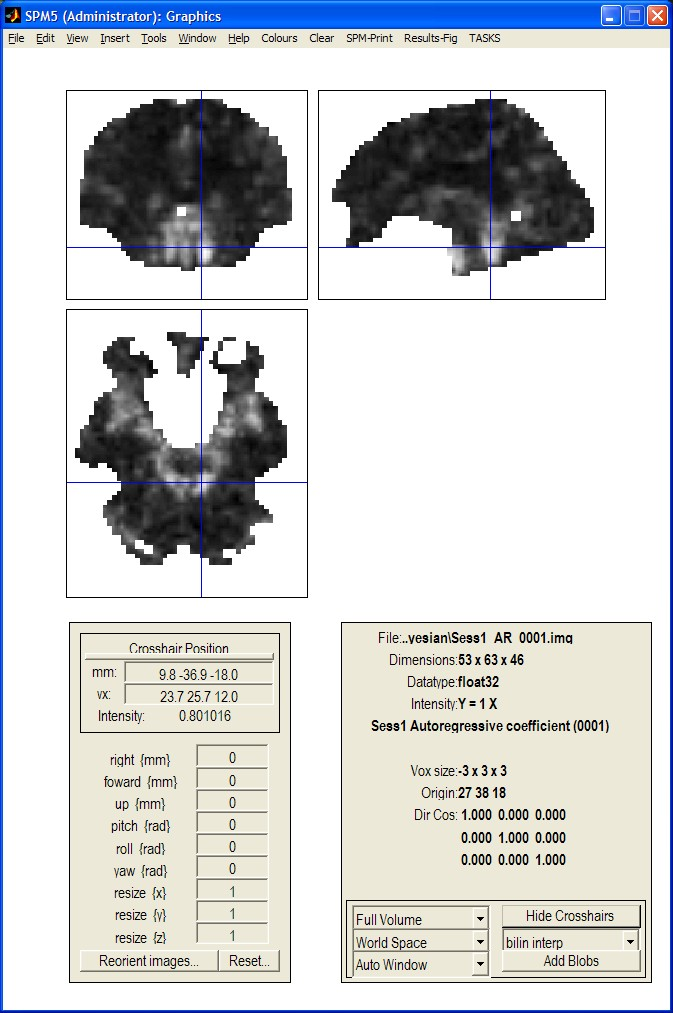
\includegraphics[width=100mm]{faces/face_ar1}
\caption{\em Bayesian analysis: Estimated AR(1) coefficient image indicating heterogeneity near the circle of Willis \label{face_ar1} }
\end{center}
\end{figure}

SPM will write a number of files into the output directory including 
\begin{itemize}
\item An \texttt{SPM.mat} file.
\item Images \texttt{Cbeta\_k.img} where $k$ indexes the $k$th estimated regression coefficient. These filenames are prefixed with a ``\texttt{C}''' indicating that these are the mean values of the ``Conditional'' or ``Posterior'' density.
\item Images of error bars/standard deviations on the regression coefficients \texttt{SDbeta\_k.img}.
\item An image of the standard deviation of the error \texttt{Sess1\_SDerror.img}.
\item An image \texttt{mask.img} indicating which voxels  were included in the analysis.
\item Images \texttt{Sess1\_AR\_p.img} where $p$ indexes the $p$th AR coefficient. See eg. Figure~\ref{face_ar1}.
\item Images \texttt{con\_i.img} and \texttt{con\_sd\_i.img} which are the mean and standard deviation of the $i$th pre-defined contrast.
\end{itemize}

\subsection{Inference}

After estimation, we can make a posterior inference using a PPM. Basically, we identify regions in which we have a high probability (level of confidence) that the response exceeds a particular size (eg, \% signal change). This is quite different from the classical inferences above, where we look for low probabilities of the null hypothesis that the size of the response is zero.

To determine a particular response size (``size threshold'') in units of PEAK \% signal change, we first need to do a bit of calculation concerning the scaling of the parameter estimates. The parameter estimates themselves have arbitrary scaling, since they depend on the scaling of the regressors. The scaling of the regressors in the present examples depends on the scaling of the basis functions. To determine this scaling, load the ``SPM.mat'' file and type in \matlab\ \texttt{sf = max(SPM.xBF.bf(:,1))/SPM.xBF.dt} (alternatively, press ``Design:Explore:Session 1'' and select any of the conditions, then read off the peak height of the canonical HRF basis function (bottom left)).

Then, if you want a size threshold of 1\% peak signal change, the value you need to enter for the PPM threshold (ie the number in the units of the parameter estimates) is \texttt{1/sf} (which should be 4.75 in the present case).\footnote{Strictly speaking, this is the peak height of the canonical component of the best fitting BOLD impulse response: the peak of the complete fit would need to take into account all three basis functions and their parameter estimates.}

Finally, if we want to ask where is there a signal greater than 1\% (with a certain confidence) to faces versus baseline, we need to create a new contrast that takes the AVERAGE of the parameter estimates for the canonical HRF across the four conditions (N1 to F2), rather than the default \texttt{Positive effect of condition\_1} contrast, which actually calculates the SUM of the parameter estimates for the canonical HRF across conditions (the average vs sum makes no difference for the classical statistics).

\begin{itemize}
\item Press ``Results''.
\item Select the \texttt{SPM.mat} file created in the last section.
\item Press ``Define new contrast'', enter the name ``AVERAGE Canonical HRF: Faces $>$ Baseline'', press the ``T-contrast'' radio button, enter the contrast [1 0 0 1 0 0 1 0 0 1 0 0]/4, press ``submit'', ``OK'' and ``Done''.
\item \emph{Mask with other contrast ? [Yes/No]}
\item Specify No
\item \emph{Title for comparison}
\item Enter ``AVERAGE Canonical HRF: Faces $>$ Baseline''
\item \emph{Effect size threshold for PPM}
\item Enter the value
\item \emph{Posterior probability threshold for PPM}
\item Enter the value 0.95
\item \emph{Extent threshold [0]}
\item Accept the default value
\item \emph{Plot effect size [Yes/No]}
\item Select the default ``Yes''
\end{itemize}
SPM will then plot a map of effect sizes at voxels where it is 95\% sure that the effect size is greater than 1\% of the global mean.
Then use overlays, sections, select the normalised structural image created earlier and move the cursor to the activation in the left hemisphere. This should create the plot shown in Figure~\ref{face_bayes}.

\begin{figure}
\begin{center}
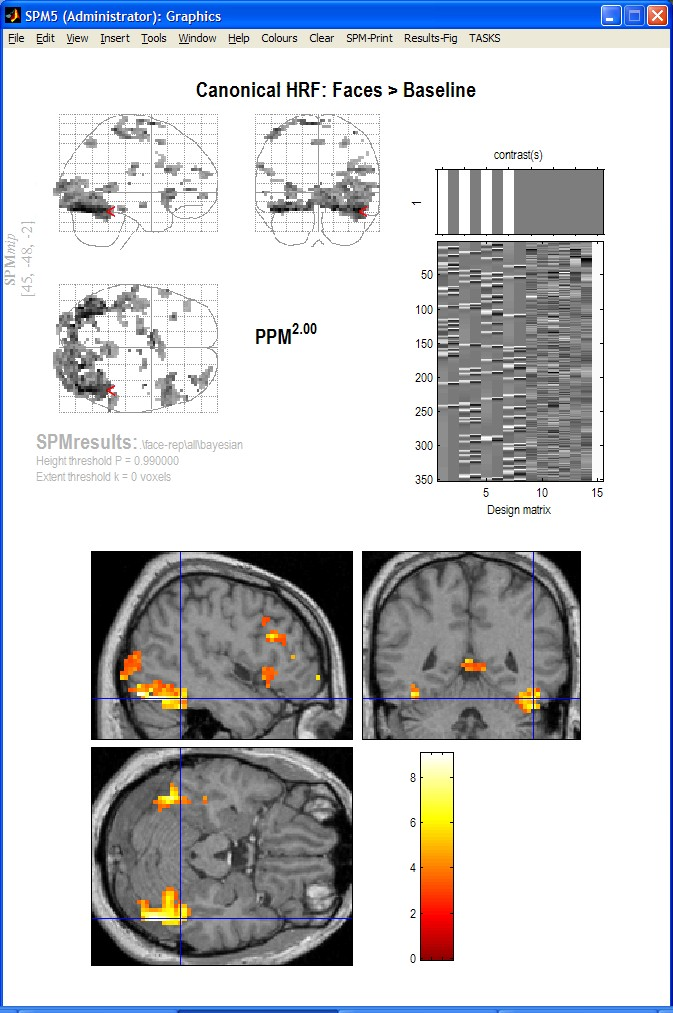
\includegraphics[width=100mm]{faces/face_bayes}
\caption{\em Bayesian analysis: MIP and overlay of effect sizes at voxels where PPM is 95\% sure that the effect size is greater than 1\% of the global mean. The cursor is at the location $x=30,y=-82,z=-17$mm\label{face_bayes} }
\end{center}
\end{figure}
